\documentclass{beamer}
\usepackage{animate}
\usepackage{tikz}

\usetikzlibrary{decorations.markings}

\newcounter{angle}
\setcounter{angle}{0}

\begin{document}

\begin{frame}[fragile]{Production of AC current}{Alternator}
\begin{center}
\begin{animateinline}[loop,poster=first,controls]{10}
    \whiledo{\theangle<720}{
        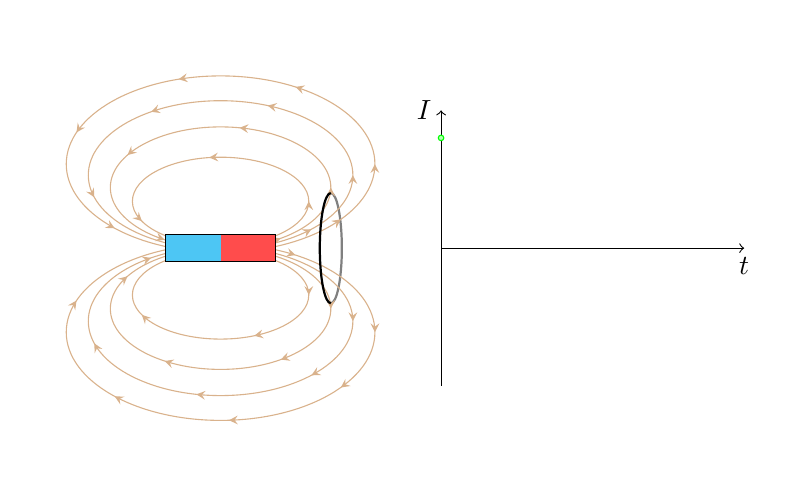
\begin{tikzpicture}[scale=.7]
        \path[use as bounding box] (-3.5,-4) -- (10,4);
        %\draw (-3.5,-4) rectangle (10,4);
        % 1/2 surface inf
        \draw[black!50,thick] (2,-1) 
            arc[start angle=-90,end angle=90,x radius=.2cm, y radius=1cm];
        \begin{scope}[rotate=\theangle]
        % lignes de champ
        \foreach \h/\X/\Y in {.85/1.6/.8, 1.1/2/1.1, 1.325/2.4/1.35,%
                1.525/2.8/1.6} {
            \draw [decoration={markings,
                    mark=between positions 0 and 1 step 1.5cm 
                        with {\arrow{stealth}}},    
                    postaction={decorate},color=brown!60] (0,\h) 
                circle[x radius=\X cm,y radius=\Y cm];
            \draw [decoration={markings,
                    mark=between positions 0 and 1 step 1.5cm 
                        with {\arrowreversed{stealth}}},    
                    postaction={decorate},color=brown!60] (0,-\h)
                circle[x radius=\X cm,y radius=\Y cm];
        }
        \end{scope}
        % 1/2 surface sup
        \draw[thick] (2,-1) 
            arc[start angle=-90,end angle=-270,x radius=.2cm,%
                    y radius=1cm];
        % aimant
        \begin{scope}[rotate=\theangle]
        \fill[color=cyan!70] (-1,-.25) rectangle (0,.25);
        \fill[color=red!70] (0,-.25) rectangle (1,.25);
        \draw (-1,-.25) rectangle (1,.25);
        \end{scope}

        % calculation of the position       
        \pgfmathrad{\theangle}
        \edef\myangle{\pgfmathresult}
        \pgfmathparse{4 + .4 * \myangle}
        \edef\myX{\pgfmathresult}
        \pgfmathparse{2 * cos(\theangle)}
        \edef\myY{\pgfmathresult}

        \coordinate (O) at (4,0);
        \begin{scope}
        % axes
        \draw[->] (O) -- ++(5.5,0) node[below]{$t$};
        \draw[->] ([yshift=-2.5cm]O) -- ([yshift=2.5cm]O) node[left]{$I$};
            \begin{scope}[xshift=4cm,xscale=0.4] % sinusoïde
            % calcul clip
            %\node at (1,1) { \myangle };
            \clip (0,-2.5) rectangle (\myangle,2.5);
            \draw[green,thick] (0,2) cos (1.5708,0) sin (3.1416,-2)
                    cos (4.7124,0) sin (6.2832,2) cos (7.8540,0)
                    sin (9.4248,-2) cos (10.9956,0) sin (12.5664,2); 
            \end{scope}

        \draw[fill=green!30,draw=green] (\myX,\myY) circle[radius=.5mm];
        \end{scope}
        \end{tikzpicture}       
        %
        %\addtocounter{angle}{720}
        \addtocounter{angle}{5}
        %\stepcounter{angle}
        \ifthenelse{\theangle<720}{%
            \newframe
        }{%
            \end{animateinline}
        }
    }
\end{center}
\end{frame}

\end{document}